\documentclass[11pt]{article}
\usepackage[utf8]{inputenc}
\usepackage[english, german]{babel}
\renewcommand{\baselinestretch}{1.05}
\usepackage{amsmath,amsthm,verbatim,amssymb,amsfonts,amscd, graphicx}
\usepackage{graphicx}
\topmargin0.0cm
\headheight0.0cm
\headsep0.0cm
\oddsidemargin0.0cm
\textheight23.0cm
\textwidth16.5cm
\footskip1.0cm
\setlength\parindent{0pt}
\theoremstyle{plain}
\newtheorem*{theorem}{Theorem}
\newtheorem*{beispiel}{Beispiel}
\newtheorem*{lemma}{Lemma}
\newtheorem*{satz}{Satz}
\newtheorem*{definition}{Definition}
\renewcommand*{\proofname}{Beweis}
\newcommand{\R}{\mathbb{R}}
\newcommand{\Q}{\mathbb{Q}}
\newcommand{\C}{\mathbb{C}}
\newcommand{\N}{\mathbb{N}}
\renewcommand{\i}{\mathrm{i}}
\newcommand{\e}{\mathrm{e}}
\newcommand{\norm}[1]{\left\Vert #1 \right\Vert}
\newcommand{\abs}[1]{\left| #1 \right|}
\newcommand{\diam}{\mathrm{diam}}
\newcommand{\dd}[2]{\frac{d{#1}}{d{#2}}}
\newcommand{\pd}[2]{\frac{\partial #1 }{\partial #2}}
\newcommand{\trace}{\operatorname{Tr}}
\newcommand{\oo}{\infty}
\newcommand{\Forall}{\quad\forall\,}
\renewcommand{\d}[1]{\,d#1\,}
\usepackage{braket}
\usepackage{centernot}

% \renewcommand{\labelitemi}{$\blacktriangleright$}
% \renewcommand{\labelitemii}{$\vartriangleright$}
% \renewcommand{\labelitemiii}{$\bowtie$}
% \renewcommand{\labelitemiv}{$\star$}
\newcommand{\sumint}{\ooalign{$\textstyle\sum$\cr\hidewidth$\displaystyle\int$\hidewidth\cr}}

\usepackage{enumerate}
\usepackage[pdf]{pstricks}
\usepackage{epsfig}
\usepackage{pst-grad} % For gradients
\usepackage{pst-plot} % For axes
\usepackage{siunitx}
\usepackage{varwidth}
\newenvironment{centerall}
{\begin{center}\begin{varwidth}{\textwidth}}
{\end{varwidth}\end{center}}

% \usepackage{MnSymbol}
\begin{document}
\section{Einf\"uhrung}
\begin{description}
  \item Makroskopische systeme aus $N \ll $ Teilchen.
  \item Mikrozustand und mikroskopische Gesetze
    \begin{itemize}
      \item Klassische Physik: 
        \[\text{Punkt } (\vec{r}, \vec{p}) \in \text{ Phasenraum} \simeq \R^{6N} \]
        \[ m_1 \ddot{\vec{r}} = \vec{F}_1 \]
      \item Quantenmechanik: 
        \[ \text{Wellenfunktion } \Psi (\vec{r},t) \in \mathcal {L}_2 (\R^{3N}) \]
        \[ i \hbar \pd{\Psi}{t}= H \Psi \]. 
    \end{itemize}
    
  \item Makrozustand und Makroskopische Gesetze
    \begin{itemize}
      \item Temperatur $T$, Volumen $V$, Druck $P$, ...
      \item $P V=nk_BT, \quad V=RI$
    \end{itemize}
  \item Mikroskopische Gesetze $\implies $ makroskopische Gesetze.
  \item Makrozustand $\iff $ Zeitmittelung
    \begin{itemize}
      \item Klassische Physik: \[ \bar{A}(t)= \frac{1}{\Delta t} \int_{t}^{\Delta t +t} dt
        A(\vec{r}(t),\vec{p}(t))\] 
      \item Quantenmechanik: \[ \bar{B} = \frac{1}{\Delta t} \int_{t}^{\Delta t+t} dt
        \Braket{\Psi(t) | \hat{B} | \Psi (t)}\] 
    \end{itemize}
  \item Mikroskopische Zeitskala $\ll\, \Delta t \, \ll$ makroskopische Zeitskala
  \item Statistische Mittelung
    \begin{itemize}
      \item Klassische Physik \[ \bar{A} = \int_{}^{} d^3r n d^3p A(\vec{r}, \vec{p}),
        \quad P(\vec{r}, \vec{p}) \text{ Wahrscheinlichkeitsdichte } P \] 
      \item Quantenmechanik: \[ \bar{B}= \operatorname{Sp}(\hat{B} \hat{P})
          \text{ Dichteoperator } \hat{P} \]   
    \end{itemize}
  \item Statistische Physik
    \begin{itemize}
      \item Bestimmung von $P$ und $\hat{P}$
      \item Berechnung der Ensemblemittelung
      \item Anwendung auf physikalische Probleme
    \end{itemize}
  \item Reduktionismus \[ \text{System } = \left\{ \text{Einzelteile} \right\} \] 
    %TODO: make this a flow diagram
  \item Elementarteilchenphysik $\to $ Festk\"orperphysik, Chemie $\to $
    Biologie $\to $ Medien $\to $ Psychologie $\to $ Soziologie
  \item ``\emph{More is different}'' P.W. Anderson
    %TODO: add pictures of snowflakes
    
\end{description}
\section{Wahrscheinlichkeitstheorie}
\emph{Schwabl Kapitel 1.2, 15.1} \\
\begin{description}
  \item [Einige Definitionen]

  \item [Zufallsvariable $x$] Wert von $x$ h\"angt von einem Zufallsereignis ab
    Beispiel Messung: $x= X_{\text{exakt}} + \text{ Messfehler }$

  \item[H\"aufigkeit] 
    $N$ identische Versuche, $N_x = \text{ Anzahl der Werte } x \implies \frac{N_x}{N}$

  \item[Empirische Wahrscheinlichkeit]
    $P_x = \lim_{N \to \inf } \frac{N_x}{N}$.
    \[ \sum_{x}{} P_x = 1 , \quad 1 \ge P_x \ge 0 \quad \] 

  \item[Wahrscheinlichkeitsdichte] 
    $w(x) \quad x \in \R$. \[ w(x)\Delta x = \text{ Wahrscheinlichkeit f\"ur einen
      Wert } \in [x, x+\Delta x]  \] 
      \[ \int_{}^{}dx\, w(x)=1, \quad w(x)\ge 0 \] 
      Beziehung mit diskreter Warscheinlichkeit: 
      \[ w(x) = \sum_{i}{}P_i \delta ( x-x_i) \] 

  \item[Mittelwert/Erwartungswert]
    \[ \Braket{f(x)} = \sum_{x}{} f(x) P_x \text{ beziehungsweise } \int_{}^{}
      dx\, w(x) f(x)\] 

  \item [Schwankungsquadrat] \[ \Delta X^2 = \Braket{(x-\Braket{X})^2}
    = \Braket{X^2}- \Braket{X}^2 \quad \Delta x \Delta p \ge \hbar/2\] 
\end{description}
\subsection{Zentraler Grenzwertsatz}
Es gibt $N$ unabh\"angige aber identische Zufallsvariablen $x_i, \, i=1 , \dotsc , N$.
\[ P(x_1,\dotsc,x_N)= P(x_1) P(x_2) \ldots P(x_N)  \]
Au\ss{}erdem existieren $\Braket{x},\Delta$ von  $P(x)$.
\[ \text{Mittelwert } Y= \frac{1}{N}\sum_{i=1}^{N}x_i  \text{ ist eine
Zufallsvariable mit Wahrscheinlichkeit } Q_N(Y) \] 
\[ Q_N(Y) \xrightarrow{N\to \inf}\frac{1}{\sqrt{2 \pi} \sigma}
\exp{(-\frac{(Y-a)^2}{2 \sigma^2})}\] 
\[ a=\Braket{x}, \quad \sigma= \frac{\Delta x}{ \sqrt{N}} \] 


\begin{figure}[htpb]
  \centering
  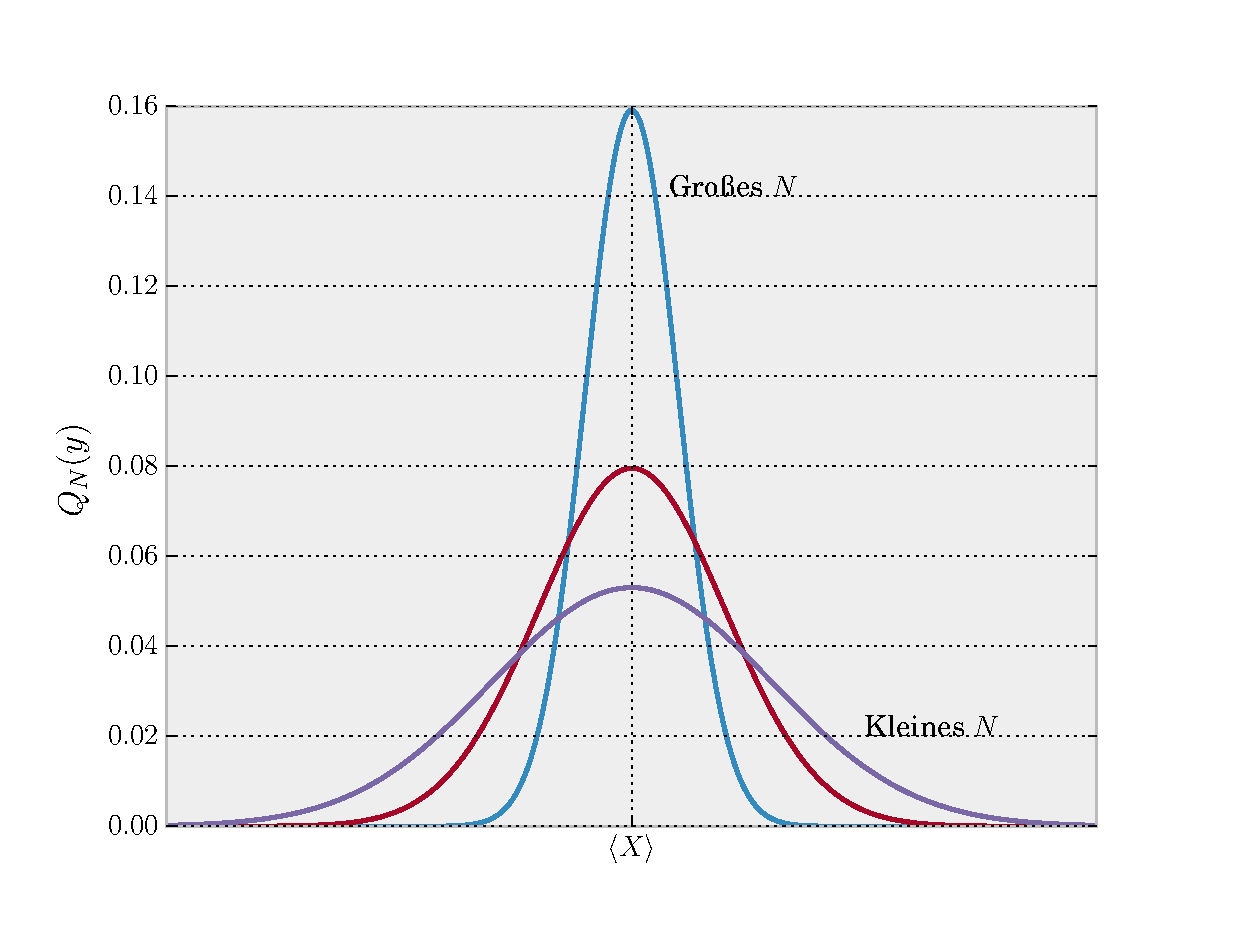
\includegraphics[width=0.8\textwidth]{./figures/first.eps}
  \caption{Normalverteilung, $Y=\Braket{X} \pm \frac{\Delta X}{\sqrt{N}} $}
  \label{fig:first}
\end{figure}
\section{Klassische Physik}
\begin{description}
  \item[N Teilchen ] Mikrozustand $(q,P) \in  \text{ Phasenraum } \simeq \R^{6n}$
  \item[Kanonische Gleichungen] \[ \dot{q}_j = \pd{H}{P_j} \quad \pd{H}{\dot{q}_j}, \quad j=1,...,3N \] 
  \item[Anfangsbedingung] \[ (q_0, P_0)= (q_0(t_0), P(t_0)) \implies \text{ Bahn } (q(t | q_0, P_0), P(t| q_0 P_0)) \] 
  \item[Kanonische Transformation ] \[ (q(t), P(t)) \iff (q(t'), P(t')) \] 
  \item[Ziel] \[ \bar{A}= \int_{}^{} d^{3N}q d^{3N}p A(q,P) P_G(q,P) \] 
    Gleichgewichtsverteilung $\rho_G(q,P)= $?
  \item[Unscharfe Angangsbedingung] \[ P(q,P,t_0)= \rho_0 (q,P) \] 
    Scharfe Anfangsbedingung: $\rho_0(q,P) = \delta(q-q_0) \delta (P-P_0)$.
    Differentialgleichung f\"ur $P(q,P,t)$: Liouville-Gleichung.
    \[ P(t)= \rho(q,P,t)d^{3N}q d^{3N}p=P(t') = \rho(q,P,t')d^{3N}q' d^{3N}p' \] 
  \item[Liouville-Satz] \[ d^{3N}q d^{3N}p = d^{3N}q' d^{3N}p' \quad \left[ \text{ Jacobi-Matrix } \frac{d^{3N}q' d^{3N}p'}{d^{3N}q d^{3N}p}= 1 \right] \] 
    \[ \implies \rho(q(t), P(t), t)= \rho (q(t'), P(t'), t'), \quad \text{ Erhalungsgroesse } \frac{dP}{dt}=0 \] 
  \item[Kettenregel] \[ \frac{d \rho(q(t), P(t),t)}{dt}= \pd{\rho}{t} + \left\{ H,P \right\} \] 
  \item[Liouville-Gleichung] \[ \pd{\rho}{t}= \left\{ P,H \right\} \] 
    Bedingungen f\"ur $\rho_G(q,P)$
    \begin{itemize}
      \item $\left\{ P_G, H \right\}=0$
      \item $P_G \ge 0$
      \item $\int_{}^{}d^{3N}q d^{3N}p \rho_G (q,P)=1$.
    \end{itemize}
    Superpositionsprinzip: L\"osungen $P_1,P_2 \implies \rho=a_1 \rho_1+ a_2 \rho_2 $
    mit $a_1,a_2 \ge 0, \quad a_1+a_2 =1$. \\
    Makrozustand: $T,V,P,... \quad  \implies \rho_0 oder \rho_g$?\\
\end{description}
\section{Quantenmechanik}

\emph{Schwabl Kapitel 1.4,1.5.2}
$N $ Teilchen, Mikrozustand $\Ket{\Psi} \in \mathcal{H} \simeq \mathcal{L}_2(\R^{3N})$
\begin{align*}
  i \hbar \frac{d}{dt} \Ket{\Psi(t)} = H \Ket{\Psi(t)} \\
  \text{Anfangsbedingung } \Ket{\Psi_0} \to \Ket{\Psi(t)} \quad \text{(eindeutig)} \\
  \text{Erwartungswert } A(t)= \Braket{\Psi(t) | \hat{A} | \Psi(t)} =\Braket{\hat{A}} \\
\end{align*}
Ziel: \[ \text{Statistische Mittelung } \quad \Braket{A} = \operatorname{Sp}(\hat{A}\hat{\rho}_G), \quad \hat{\rho=?} \] 
\subsubsection*{Definition}
Statistische Operator, Dichteoperator, Dichtematrix,...
\begin{align*}
  \hat{\rho} & : \mathcal{H} \to  \mathcal{H}, \text{ linear } \\
  \hat{\rho} & = \hat{\rho}^+ \\
  \text{positiv-semidefinit } & \Braket{\varphi | \hat{\rho}| \varphi} \ge 0 \,\forall\,\Ket{\varphi} \in \mathcal{ H} \\
  \operatorname{Sp} \hat{\rho } & =1  &
  \text{Spektrale Zerlegung } & \begin{split}
  \hat{\rho} &=  \sum_{n}^{} p_n \Ket{n}\Bra{n} \\ &= \int_{}^{} d \lambda \Ket{\lambda}\Bra{\lambda} w(\lambda) 
  \end{split}
   \\
  \text{Dichteoperator } & \implies \begin{matrix} p_n \ge 0 \\ \sum_{n}^{} p_n =1 \\
p_n \in \R \end{matrix} 
&
\begin{matrix} 
  w(\lambda )\ge 0 \\ \int_{}^{} d \lambda w( \lambda )=1 \\ w(\lambda) \in \R 
\end{matrix} \\
  \Braket{\hat{A}}= \sum_{n}^{}p_n \Braket{n|\hat{A}|n}.
\end{align*}
\begin{description}
  \item[Reiner Zustand]: \[ p_{n_0}, p_n =0 \,\forall\, n \neq n_0, \quad  \hat{\rho}= \Ket{n_0}\Bra{n_0} \implies \hat{\rho}^2=\hat{\rho} \]  
  \item[Gemisch]: $p_n \neq 0 $ f\"ur 2 oder mehr $n$.
    \begin{itemize}
      \item Verschr\"ankte Zust\"ande
      \item Statistisches Gemisch
    \end{itemize}
  \item[Spektrale Zerlegung] \begin{align*}
    \hat{A} = \sum_{\alpha}^{}a_ \alpha \Ket{\alpha}\Bra{\alpha} \\
    \Braket{A}= \sum_{n}^{}p_n \sum_{\alpha}^{}a_ \alpha \abs{\Braket{\alpha}| n}^2
    = \sum_{n}^{}\sum_{\alpha}^{} \underset{\text{Stat. Zufall}}{p_n} \underset{\text{Q.M. Zufall}}{\abs{\Braket{n|\alpha}}^2} a_ \alpha
  \end{align*}
  % TODO: Fig 4
  \[ \text{Gemisch: 2 Quellen: } I_1, \theta_1, \quad I_2 \theta_2 \implies 
  I'= I_1 ( \cos{\theta_1})^2 + I_2 (\cos{\theta_2})^2 \] 
  \[ p_1 = \frac{I_1}{I_1 + I_2}, \quad p_2 = \frac{I_2}{I_1 + I_2} \] 
\end{description}
\subsection*{Von Neumann Gleichung}
\[ i \hbar \frac{d\hat{\rho}}{dt} = \left[ H, \hat{\rho} \right] \] 
\begin{itemize}
  \item Anfangsbedingung $\hat{\rho}_0 \to  \hat{\rho}(t)$
  \item Gleichgewicht: \[ \frac{d \hat{\rho}}{dt}=0 \implies  \left[ H, \hat{\rho} \right]=0  \] 
  \item Superpositionsprinzip $\rho= a_1 \rho_1 + a_2 \rho_2 \text{ mit } a_1, a_2 \ge 0,
    \text{ und } a_1+a_2 =1 $
  \item Im Gleichgewicht: \[ \hat{\rho}_G = \sum_{n}^{} p_m \Ket{E_n}\Bra{E_n} \text{ mit }
      H \Ket{E_n}\Bra{E_n} = \int_{}^{} dE\, w(E)\Ket{E}\Bra{E} \quad \text{ mit }
    H \Ket{E}= E \Ket{E}\] 
    \[ p_n = \frac{1}{Z_n} \text{ f\"ur } E_n = E_0, \quad Z_n= \text{ Entartung des Niveaus } E_0 \] 
    % TODO: Fig 5
    \[ p_n = \frac{1}{Z} e^{-\beta E_n} \text{ mit } 
    \beta= \frac{1}{k_B T}, \quad Z=\sum_{n}^{} e^{-\beta E_n} \] 
\end{itemize}

\subsection*{Entropie und Ensemble}
\begin{description}
  \item[Definition] Entropie (Quantenstatistik) \\
    \[ S =-k_B \operatorname{Sp}(\hat{\rho} \ln{\hat{\rho}}) \quad k_B = k = 
      \text{ Boltzmann-Konstante }
    \approx \SI{1,38e-23}{\joule\per\kelvin} \] 
  \item[Eigenschaften] 
    \begin{align*}
      \hat{\rho} = \sum_{n}^{} p_n \Ket{n}\Bra{n} && p_n \ge 0 && \sum_{n}^{} p_n = 1 \\
      S(\left\{ p_n \right\}) = -k_B \sum_{n}^{} p_n \ln{p_n}
    \end{align*}
    Hinweise: \begin{align*}
      \operatorname{Sp} \hat{A} = \sum_{n}^{}\Braket{n | \hat{A}|n} && f(\hat{\rho})= 
      \sum_{n}^{} f( p_n) \Ket{n}\Bra{n} \\
      e^{\hat{A}}= \sum_{n=0}^{ \oo } \frac{1}{n!}\hat{A}^n
    \end{align*}
    Die Entropie ist also die Summe der Diagonalemente der Dichtematrix in
    diagonalisierter Form. Dies ist wohldefiniert, da jede Dichtematrix
    diagonalisiert werden kann.
    Extrema mit Nebenbedingung $\sum_{n}^{} p_n = 1$
    \begin{itemize}
      \item Minimum $S=0$ f\"ur einen reinen Zustand ($p_{n_0}=1, p_n =0
        \quad\forall\, n \neq n_0$)
      \item Maximum $S= k_B \ln{M}$ f\"ur $p_n = \frac{1}{M} \quad\forall\, 1,...,M$.
    \end{itemize}
    Die entropie ist maximal f\"ur Unkenntnis \"uber den Zustand des Systems
    (Auch ma\ss{} f\"ur Unordnung).
  \item[Extensivit\"at] \[ \mathcal{H}= \mathcal{H}_A \otimes \mathcal{H}_B,
  \quad \hat{\rho} = \hat{\rho}_A \otimes  \hat{\rho}_B \] 
  \begin{align*}
    \hat{\rho}_A \to  \hat{\rho}_A \otimes  \hat{I}_B  \\
    \hat{\rho}_{\hat{B}} \to  \hat{I}_A \otimes  \hat{\rho}_B \\
    \implies \left[ \hat{\rho}_A, \hat{\rho}_B  \right]= 0
  \end{align*}
  \begin{align*}
    S & = -k_B \operatorname{Sp} ( \hat{\rho} \ln{\hat{\rho}}) = k_B \operatorname{Sp}
    \left[ \hat{\rho}_A \hat{\rho_B} (\hat{\rho_A} = \ln{\hat{\rho}_B}) \right] \\
    & = -k_B \operatorname{Sp} (\hat{\rho}_A \ln{ \hat{\rho}_A}) - k_B \operatorname{Sp}
    (\hat{\rho}_B \ln{ \hat{\rho}_B}) = S_A + S_B
  \end{align*}
  Nebenbedingung

  \[ S \le S_A + S_B \] (z.B. verschr\"ankte Systeme)
\item[Beispiel] System von $N$ Spins $S$ ($\vec{S}^2 =  S(S+1)$). \\
  Hilbert-Raum f\"ur einen Spin $= \mathcal{H}_1 = \C^{2S+1}$.
  Gesamter Hilbert-Raum \[ \mathcal{H} = \bigotimes_{i=1}^{N} \mathcal{H}_i \] 
  \[ \operatorname{dim} \mathcal{H} = (2S+1)^N = M \] 
  \begin{itemize}
    \item Minimum $S=0$ z.B. f\"ur $\Ket{\Psi} = \Ket{ \uparrow, \uparrow, \uparrow, \ldots, \uparrow}$.
    \item Maximum $S= k_B \ln{M}$ f\"ur $\hat{\rho}= \frac{1}{n} \hat{I}=
      k_B n \ln{(2S+1)}$
  \end{itemize}
\item[Gleichgewicht]
  \begin{align*}
    0= \frac{d \rho }{dt} \iff \left[ H, \hat{\rho} \right]=0 \implies 
    \rho = \sum_{m}^{} p_n \Ket{E_n} \Bra{E_n} \\
    \implies E = \Braket{\hat{H}} = \operatorname{Sp} (\hat{\rho} \hat{H})
    = \sum_{n}^{} p_n E_n
  \end{align*}
  \begin{align*}
    \rho \Ket{E_n} = p_n \Ket{E_n} \\
    H \Ket{E_n} = E_n \Ket{E_n}
  \end{align*}
\end{description}
\begin{description}
  \item[Definition]  Statistisches Ensemble oder Gesamtheit \\
    Sie ist eine Gewichtete Menge der Mikrozust\"ande, die einen 
    Makrozustand entsprechen.
    \begin{align*}
      \left\{ ( \Ket{N}, p_n) \right\} \equiv \hat{\rho} = \sum_{n}^{} p_n
      \Ket{n} \Bra{n} 
    \end{align*}
\end{description}
\subsection*{Zentrales Postulat der statistischen Physik}
System mit $N(\to \inf{})$ Freiheitsgraden im Gleichgewicht.
\begin{itemize}
  \item $S$ ist maximal f\"ur einen gegebenen Makrozustand. Das erlaubt uns
    eine eindeutige bestimmung des statistischen Operators $\hat{\rho}$.
  \item Statistische Mittelungen der Observablen erf\"ullen die Makroskopischen
    Gesetze der Thermodynamik.
    \begin{align*}
      S = -k_B \operatorname{Sp} \hat{\rho}_B = - k_B \Braket{\ln{\hat{\rho}_G}} \\
      \Braket{\hat{\cal{O}}}= \operatorname{Sp} (\hat{\rho}_G \mathcal{O}) &&
      U = \Braket{\hat{H}}
    \end{align*}
\end{itemize}
\begin{description}
  \item[Definition] Entropie (Thermodynamik) \\
    Wir betrachten ein System in einem Bad, mit welchem es Energie austauschen
    kann. Eine ideelle Situation, in welcher alle Prozesse die wir betrachten 
    reversibel sind. 
    \begin{align*}
      dS = \frac{\delta Q}{T}
    \end{align*}
    Zustandsfunktion oder Thermodynaische Variable.
    \begin{itemize}
      \item Extensiv
      \item monoton steigend $\pd{S}{E} > 0$
      \item $ \lim_{T \to 0} \frac{S}{N} = 0$.
    \end{itemize}
\end{description}
\begin{description}
  \item[Nebenbedingung] F\"ur bestimmte Modelle statistische Entropie nicht
    gleich der thermodynamischen Entropie, das bedeutet das Modell ist nicht
    physikalisch. Eigentlich hat man in den letzten 100 Jahren in denen man
    Forschung betreibt kein Problem gefunden, das man nicht l\"osen konnte.
    Es gibt verschiedene Situationen in derr Praxis, in denen man die Makrozust\"ande
    beschreibt. 
\end{description}
\subsection*{Mikrokanonisches Ensemble}
Es beschreibt ein isoliertes System.
\begin{description}
  \item[Freie thermodynamische Variablen] $ $ 
    \begin{itemize}
      \item Teilchenzahl $N$
      \item Volumen $V$
      \item Magnetisierung $M$
      \item Energie $E$
    \end{itemize}
  \item[Zustandsfunktion] Druck $P(N,V,E)$
  \item[Maximierung der Entropie] 
    \begin{align*}
      \hat{\rho} & = \subset P_E P_N \ldots \\
      \hat{\rho} & ~ \delta(\hat{H} - E) \delta (\hat{N} - N)
    \end{align*}
\end{description}
\subsection*{Kanonisches Ensemble}
Beschreibt ein geschlossenes System.
\begin{description}
  \item[Freie thermodynamische Variablen] $ $
    \begin{itemize}
      \item Temperatur $T$
      \item $N, V, M$
    \end{itemize}
  \item[Zustandsfunktionen] $E(T, N, V)$
  \item [Maximum der Entropie] 
    F\"ur feste $T, N, V, \ldots$
    \begin{align*}
      \hat{\rho} = \frac{1}{z} e^{- \beta \hat{H} } \hat{P}_N \ldots && 
      \beta = \frac{1}{k_B T}
    \end{align*}
  \item[Zustandsumme]
    \begin{align*}
      z= \operatorname{Sp} e^{- \beta \hat{H}}
    \end{align*}
\end{description}


\subsection*{Gro\ss{}kanonisches Ensemble}
Beschreibt ein offenes System
\begin{description}
  \item[Freie Thermodynamische Variablen]  $ $
    \begin{itemize}
      \item Chemisches Potential $\mu$
      \item $T, V, \ldots$
    \end{itemize}
  \item[Zustandsfunktionen] $N(T, \mu, V)$
  \item[Maximum der Entropie] f\"ur feste $T, \mu, V$ falls
    \begin{align*}
      \hat{\rho}_G = \frac{1}{Z_{GK}} e^{-\beta(\hat{H}- \mu \hat{N})} P
    \end{align*}
  \item[Gro\ss{}kanonische Zustandssumme] $Z_{GK} 
    \operatorname{Sp} e^{-\beta(\hat{H}- \mu \hat{N})} $
\end{description}
\subsection*{Viele weitere Ensembles}
Zu jeder intensiven Variable gibt es eine Extensive Variable(Observable).
 \begin{align*}
   \underset{\text{Intensive Variable}}{ \text{(\"au\ss{}eres Feld)}} &<->& 
   \underset{Extensive Variable}{\text{Observable}}
   y && x \\
   \hat{\rho}_G ~ e^{- \beta y \hat{x}} && \hat{\rho}_G ~ 
   P_x ~ \delta (\hat{x} -x ) \\
   \text{Beispiele}
   M && N \\
   P && V \\
   H && M \\
   \text{(Magnetfeld)} && \text{(Magnetisierung)} \\
 \end{align*}
 




 \section*{Mikrokanonisches Ensemble}
 Wir betrachten ein isoliertes System. Zum beispiel ein Gas in einem Beh\"alter
 welcher isoliert ist. Energie und Teilchenzahl sind fest. Genauso das Volumen.
 Eine \"Ahnliche Situation w\"are auch ein magnetisches Material. Die isolation
 w\"are hier ein Material welches keine magnetischen Felder durchl\"asst.
 Typisch f\"ur das isolierte System ist, dass die Energie eine kontrollierbare
 Variable ist.

 Es gibt also eine Freie thermodynamische Variable $E$. Die erlaubten 
 Mikrozust\"ande sind die Eigenzust\"ande des Hamilton-Operators $H$ zur
 Energie $E$.
 Das Ziel ist nun die mikrozust\"ande zu beschreiben und die makroskopischen
 Variablen zu berechnen. Man braucht dazu den statistischen Operator.
 \begin{description}
   \item[Diskretes Eigenspektrum] 
     \begin{align*}
       \hat{\rho} = \sum_{n}^{} p_n \Ket{n}\Bra{n} \quad : \quad \mathcal{H} \to 
       \mathcal{H} && p_n =0 \quad\forall\, n \text{ mit } E_n \neq E \\
       \hat{\rho}= \sum_{n=1}^{w(E)} p_n \Ket{n}\Bra{n} &&
       w(E) = \text{ Entartung der Eigenergie } E
     \end{align*}
     Wir verwenden das Postulat der maximierung der Entropie:
     % \begin{align*}
     %   S(E)= -k_B \sum_{n=1}^{w(E)} p_n \ln{p_n}, && 
     %   \sum_{n=1}^{w(E)} p_n = 1 
     % \end{align*}
     \begin{align*}
       0  &= \pd{S}{p_n} - \lambda \pd{}{p_n} 
       \left( \sum_{n=1}^{w(E)} p_m -1 \right)  \\
       & = -k_B \left( \ln{p_n} +1 \right) - \lambda \Forall 1 ,\dotsc, w(E) \\
     \end{align*}

     \begin{align*}
       \text{ Extrema f\"ur }      
       & \implies p_n = e^{-\frac{\lambda}{k_B} - 1} \implies p_n = \frac{1}{w(E)} \\
       & \implies S(E) = k_B \ln{(w(E))} \text{ ist auch ein Maximum }
     \end{align*}

   \item[Dichteoperator im Gleichgewicht]
     \begin{align*}
       \hat{\rho}_G = \sum_{n=1}^{w(E)} \frac{1}{w(E)} \Ket{n}\Bra{n} =
       \frac{1}{w(E)} P_E = \frac{1}{w(E)} \delta(H-E) & \\
     \end{align*}
     \begin{align*}
       \trace \hat{\rho}_G = 1 && \trace P_E = w(E) \\
     \end{align*}

   \item[Kontinuierliches Spektrum]
     \begin{flalign*}
       \hat{\rho} &= \int_{}^{} d\lambda\, \Ket{\lambda}\Bra{\lambda} p(\lambda) \\
       N(E) &= \text{ Anzahl der Zust\"ande mit einer Eigenenergie } \le E
     \end{flalign*}
     Hinweis: F\"ur ein diskretes System von Eigenzust\"anden
     f\"ur ein kontinuerliches Spektrum kann man die Anzahl der Eigenzust\"ande 
     kleiner Als $w$ definieren.
     \begin{align*}
       w(E) &= \frac{dN}{dE} = \text{ Zustandsdichte } \\ & \implies w(E) \Delta E
       = \text{ Anzahl der Eigenzust\"ande in } \left[ E, E+ \Delta E \right] \\
       S(E) &= k_B \ln{(w(E) \Delta E)} \\
       \hat{\rho} &= \frac{1}{w(E)} \delta(H-E) 
     \end{align*}
 \end{description}
 \subsection*{Thermodynamische Variablen}
 Man macht eine Statistische Mittelung
 \begin{align*}
   \Braket{\hat{\cal{O}}} = \trace (\hat{\rho}_G \hat{\cal{O}})
 \end{align*}
 \begin{description}
   \item[Beispiele] 
     \begin{align*}
      \text{Innere Energie: } U= \Braket{H} = E \\
      \text{Magnetisierung: } M_z = \Braket{S_z} \\
     \end{align*}
   \item[Thermodynamischer Limes] ($N \to \infty$)
   \item[Definition:] Temperatur
     \begin{align*}
       \frac{1}{T} = \left( \pd{S}{E} \right)_x
     \end{align*}
   \item[Definition] Konjugierte Variablen \\
     Beispiele: 
     \begin{align*}
     x = \begin{bmatrix} M \iff  H \\ N \iff  M \\ V \iff P \end{bmatrix} y
     \end{align*}
     \begin{align*}
       S(E,X), && y= \pm  T \left( \pd{S}{X} \right)_E
     \end{align*}
   \item[Statistische Physik] $ $ \\
     \begin{align*}
       \text{Observable } \hat{x}, \quad \text{ extensiv }, && [\hat{x}, \hat{H}]
       \xrightarrow{ N \gg 1} N^0, n^{-1} \\
       \implies \Braket{\hat{x}} = x && S(E,X) = k_B \ln{ w(E,X)} \\
     \end{align*}
 \end{description}
\subsection*{Beispiel: System von nicht-wechselwirkenden Spins}
\begin{align*}
  N \text{ Spins } s=1, && H = \sum_{i=1}^{ N } H_i = J \sum_{i=1}^{N} S_{iz}^z
  \quad (J>0) \\
\end{align*}

Eigenzust\"ande: 

\begin{align*}
  \text{1 Teilchen } & \begin{cases}
    H_i \Ket{M_j} = J S_{j z}^z \Ket{m_j} = J \hbar^2 m_j^2 \\
    S_{zj} \Ket{m_j} = \hbar m_j \Ket{m_j} &  m _j = -1,0,1 \\
  \end{cases} \\
  \text{$N$ Teilchen } & \begin{cases}
    \text{Dim } \mathcal{H} = 3^N \\ %REALLY? \\
    \Ket{ \left\{ m_j \right\} }= \Ket{m_j} \otimes \Ket{m_j} \otimes  \ldots 
      \otimes  \Ket{m_N} \\
      E(\left\{ M_j \right\})= J \sum_{j=1}^{N}m_j^2 \\
      S_z \Ket{ \left\{ m_j \right\} }= {\sum_{j}^{} m_j } & M=\sum_{j}^{}
      m_j
      \Ket{ \left\{ m_j \right\} }
  \end{cases} \\
  & H\Ket{ \left\{ m_j \right\} } = E (\left\{ m_j \right\}) \Ket{ \left\{ m_j \right\} }
\end{align*}

\begin{description}
  \item[Problem]  Entartung $w(E,M)$ \\
    \begin{align*}
      N_+ & = \text{ Anzahl der Spins mit } m_j = +1 \text{ in } \left\{ m_j \right\}\\
      N_0 & = \text{ Anzahl der Spins mit } m_j = +0 \text{ in } \left\{ m_j \right\}\\
      N_- & = \text{ Anzahl der Spins mit } m_j = -1 \text{ in } \left\{ m_j \right\}\\
    \end{align*}

    \begin{align*}
      \implies \begin{cases}
        E = J (N_+ + N_-) \\
        M = N_+ - N_- \\
        N = N_+ +N_- + N_0 \\
      \end{cases}
      \implies \begin{cases}
        N_+ = \frac{R+M}{L} =  \frac{r+m}{ L}N \\
        N_- = \frac{R-M}{L} = \frac{r - m}{ L} N\\
        N_0 = N-R = (1- r ) N \\
      \end{cases}
    \end{align*}

    \begin{align*}
      \text{Energie pro Spin ist } r= \frac{R}{N}= \frac{E}{NJ} \quad \in [0, 1] \\
      \text{Magnetisierung pro Spin } m = \frac{M}{N} \quad \in [-1, 1]
    \end{align*}

    Problem: $N_+$ unterscheidbare Zust\"ande $m_j= +1$ auf $N$ Spins verteilen.

    \begin{align*}
    & \implies \begin{pmatrix} N \\ N_+ \end{pmatrix} = \frac{N!}{N_+!(N-N_+)!}
      \text{ M\"oglichkeiten }  \\
      \end{align*}

      Danach: $N_-$ unterscheidbare Zust\"ande auf $N-N_+$ Spins mit
      $m_j = -1$ verteilen.
      \begin{align*}
      \implies \begin{pmatrix} N-N_+ \\ N_- \end{pmatrix} \text{ Moeglichkeiten} 
      \end{align*}

      Also insgesamt:
      \begin{align*}
       w(E,M) & = w(N_+, N_-) \\
      & = 
      \begin{pmatrix} N \\ N_+ 
      \end{pmatrix}  
      \begin{pmatrix} N-N_+ \\ N_- 
      \end{pmatrix} \\ & = \frac{N!}{N_+! N_-! N_0!} 
      \end{align*}

      Damit folgt die Entropie:
      \begin{align*}
        \begin{split}
         S(E,M) & = S(N_+, N_-) \\ &= k_B \ln{}\left( 
        \frac{N!}{N_+! N_-! N_0! }\right) 
      \end{split}
    \end{align*}
  Annahme: $N, N_+, N_0, N_- \gg 1$ aber
    
    \begin{align*}
      & \frac{N_+}{N}, \frac{N_-}{N}, \frac{N_0}{N} \text{ fest und endlich } \\
      \iff & m,n \text{ fest und endlich} \\
      \iff & M,E \text{ sind extensiv } (M,E \propto N)
    \end{align*}
    Stirling Formel \begin{align*}
      & \ln{N!} \approx N \ln{N} - N \\
      \implies & S(E, M) = k_B N f(r, m) \\
      f(r, m ) & = - \left[ \frac{r+m}{2} \ln{(r+m)} + \frac{r - m}{2}
    \ln{\frac{(r - m)}{2}} + (1-r) \ln{(1 - r)} \right]
    \end{align*}
  \item[Temperatur]
    \begin{align*}
      \frac{1}{T} = \left( \pd{S}{E}  \right)_M = \frac{k_B}{J} 
      \ln{\left( \frac{2 (1-r)}{ \sqrt{r^2 - m^2}} \right)}
    \end{align*}
  \item[Ohne Magnetisierung] $M=0$ genau dann, wenn $m=0$.
    \begin{align*}
      S(E) = - k N [ r \ln{\frac{r}{2}} + (1-r) \ln{(1-r)}] \\
    \end{align*}
    %
    \begin{align*}
      \frac{1}{T} = \frac{k_B}{ J } \ln{\left( \frac{2 ( 1-r)}{r} \right) }
       \begin{cases}
         > 0 & \text{ falls } 0 < r < \frac{2}{3} \\
         < 0 & \text{ falls }\frac{2}{3} < r < 1 \\
      \end{cases}
    \end{align*}
    \begin{align*}
      \implies  r (T) &= \frac{2}{e^{\beta J }+2 }, \quad  \beta= \frac{1}{k_B T} \\
                E(T)  &= NJ \frac{2}{e^{\beta J}} \frac{2}{e^{\beta J} + 2} \\
                S(T)  &= k N \left[ \frac{2}{e^{\beta J} + 2} \ln{(e^{\beta J} + 2)}
    - \frac{1}{e^{-\beta J} + 2} \ln{ \left( 1+ 2 e^{-\beta J} \right) }\right]
    \end{align*}
  \item[Diskussion] $ $  \\
    Tiefe Temperaturen \begin{align*}
      k_B T \ll J \iff \beta J \longrightarrow \infty \quad \implies \begin{cases}
        E \longrightarrow 0 \\ S \longrightarrow 0
      \end{cases}
    \end{align*}
    Nebenbedingung f\"ur $J < 0$: 
    \begin{align*}
      \implies  \begin{cases}
        E = N J \\
        S = k_B N \ln{(z)}
      \end{cases}
    \end{align*}

    Hohe Temperatur $k_B T \gg J$

    \begin{align*}
      \iff \beta J \longrightarrow  0 \implies 
      \begin{cases}
        E = \frac{2}{3} N J \\
        S = \frac{1}{3} k_B N \ln{(3)}
      \end{cases}
    \end{align*}
\end{description}
\end{document}
